\documentclass[preprint,3p,twocolumn,times,authoryear]{elsarticle}

\usepackage{wrapfig}
\usepackage[font=small]{caption}
\usepackage{subcaption}
\usepackage{amsmath}
\usepackage{geometry}
\usepackage{url}
\usepackage{booktabs}
\usepackage{multirow}
\usepackage{stfloats}

\DeclareMathOperator\erf{erf}

%%%%%%%%%%%%%%%%%%%%%%%
%% Elsevier bibliography styles
%%%%%%%%%%%%%%%%%%%%%%%
%% To change the style, put a % in front of the second line of the current style and
%% remove the % from the second line of the style you would like to use.
%%%%%%%%%%%%%%%%%%%%%%%

%% Numbered
%\bibliographystyle{model1-num-names}

%% Numbered without titles
%\bibliographystyle{model1a-num-names}

%% Harvard
\bibliographystyle{model2-names}\biboptions{authoryear}

%% Vancouver numbered
%\usepackage{numcompress}\bibliographystyle{model3-num-names}

%% Vancouver name/year
%\usepackage{numcompress}\bibliographystyle{model4-names}\biboptions{authoryear}

%% APA style
%\bibliographystyle{model5-names}\biboptions{authoryear}

%% AMA style
%\usepackage{numcompress}\bibliographystyle{model6-num-names}

%% `Elsevier LaTeX' style
%\bibliographystyle{elsarticle-num}
%%%%%%%%%%%%%%%%%%%%%%%

\journal{Icarus}

\begin{document}

\begin{frontmatter}

\title{A comparison of the Block and Full Acoustic Fluidization Models}

\author[label1]{Hamish C. F. C. Hay}
\author[label2]{Gareth S. Collins}
\author[label2]{Tom M. Davison}
\address[label1]{Lunar and Planetary Laboratory, University of Arizona, Tucson, AZ 85719, United States}
\address[label2]{Impacts and Astromaterials Research Centre, Department of Earth Science and Engineering, Imperial College London, London, SW7 2BP, United Kingdom}

\begin{keyword}
impact processes\sep cratering
\end{keyword}

\begin{abstract}

\noindent During the collapse of large impact craters, an extraordinary degree of rock weakening occurs. Current models fail to predict localised weakening, thus only broad-scale crater characteristics are reproduced. Acoustic fluidization is a physical mechanism that describes localised weakening via the action of acoustic vibrations. In this work, the iSALE impact cratering hydrocode is successfully modified to include the full Melosh model of acoustic fluidization. A comparison between the Melosh model and a widely used alternative, the block model, was carried out. The two models were found to be most similar for generation of simple craters; however, complex crater collapse in the block model is facilitated  by a deep weakening, whereas shallow weakening results in crater collapse for the Melosh model. The Melosh model of acoustic fluidization is shown to be an effective model of dynamic weakening, differing from the block model by its style of crater collapse and peak ring formation.

\end{abstract}
\end{frontmatter}

\newpage
\section{Introduction}

\hbadness=10000
\vbadness=10000

Impacts craters are the dominant landform on the majority of the terrestrial planets. Despite this, there are no eye-witness accounts of crater formation on Earth. 

Forming an impact cratering is a process that not only affects surface morphology, but also strongly influences the evolution of life. For example, it is now widely accepted that a large impact at Chicxulub, Mexico, was the prime reason for the mass extinction event at the Cretaceous-Palaeogene boundary, 66 Ma \citep{schulte2010chicxulub}.

Numerical modelling is a powerful tool for understanding impact crater formation. Model results can be compared to observed crater characteristics, revealing a great deal about the impactor itself, such as its diameter, velocity, angle of impact, and kinetic energy. It is impossible to accurately predict these characteristics from field observations alone. 

During the formation of large impact craters the target rock undergoes a remarkable drop in yield strength relative to static rock measurements. A result of this low yield strength is the formation of a collapsed, terraced crater rim and a central peak/peak ring (Figure \ref{fig:mercurycrater}, \ref{fig:lunarcrater}). Several different models of dynamic weakening attempt to explain this drop in yield strength \citep{kenkmann2012modification}. The aim of this work is to compare and contrast two of these models, the \textit{block oscillation model} \citep{ivanov1997block}, and the \textit{full model of acoustic fluidisation} \citep{melosh1979acoustic}.

The block model is itself well tested \citetext{\citet{collins2002hydrocode} and \citet{morgan2000peak}, for example}. For sufficiently large impacts, the block model generates a collapsed rim and central peak/peak ring. However, the weakening generated by the block model is broad and unlocalised. As a result, discrete, terraced fault blocks are never produced, and so current simulations only accurately recreate the broad-scale features of impact crater morphology. 

The full Melosh model of acoustic fluidisation does predict localised weakening through the action of acoustic vibrations \citep{melosh1979acoustic}, and thus may be able to reproduce the localised as well as the broad-scale features of complex craters.

To fully understand the results presented in this work, it is prudent to briefly review the impact process.

\subsection{The Cratering Process}

The process of forming an impact crater is broadly subdivided into three sections; (1) \textit{contact and compression}, (2) \textit{excavation}, and (3) \textit{modification} \citep{osinski2012impact}. 

Contact and compression begins when the impactor makes contact with the surface of the target. Kinetic energy from the impactor is transferred into the target, resulting in both melting/vaporisation and excavation of material near the point of impact \citep{melosh2012contact}. This begins the excavation stage, where material is radially ejected away from the point of impact. Excavation ends when the outward flow of material ceases \citetext{e.g., \citet{osinski2012impact}}. The last stage, modification, is crucial in determining the final crater morphology.

\begin{figure*}[!t]
\begin{minipage}[t]{0.32\linewidth}
\centering
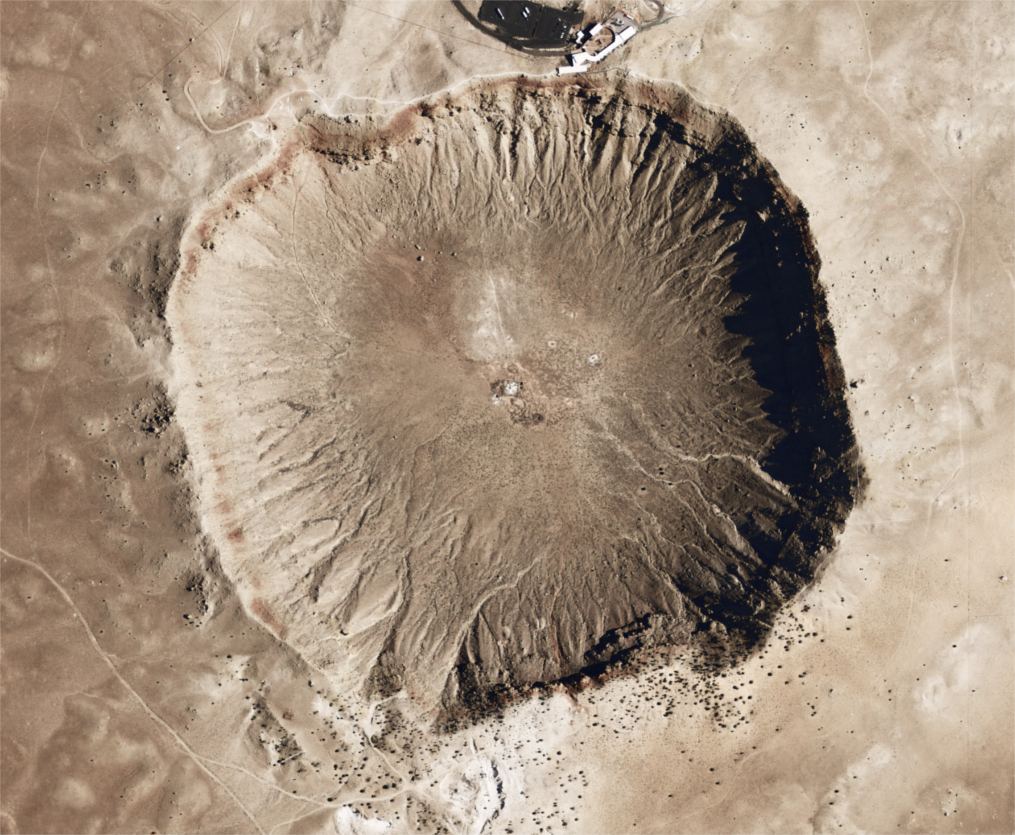
\includegraphics[width=\linewidth]{images/meteor_crater_crop.png}
\subcaption{\textit{Meteor Crater, Arizona}. A classic example of a simple crater on Earth, with a diameter of approximately 1.2km. Image from NASA's aircraft camera instrument. Image credit: NASA Earth Observatory. \url{http://earthobservatory.nasa.gov/IOTD/}. Accessed on December 2nd, 2013. \label{fig:meteorcrater}}
\end{minipage}\hspace*{\fill}
\begin{minipage}[t]{0.32\linewidth}
\centering
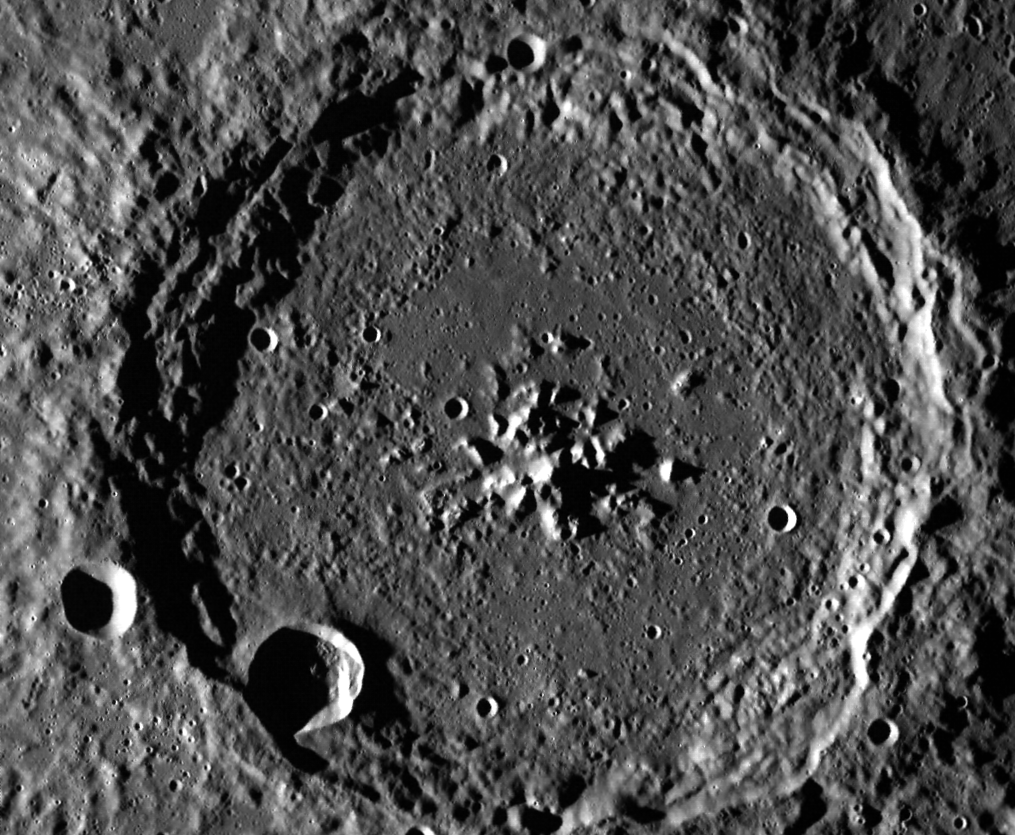
\includegraphics[width=\linewidth]{images/mercurycomplexcrater.png}
\subcaption{\textit{Verdi Crater, Mercury}. A complex crater on the surface of Mercury with a diamater of approximately 144km \citep{hale1980central}. Notice the central peak and collapsed, terraced rim. Image from NASA's Messenger MDIS instrument. Image credit: NASA. \url{http://photojournal.jpl.nasa.gov/}. Accessed on December 2nd, 2013. \label{fig:mercurycrater}}
\end{minipage}\hspace*{\fill}
\begin{minipage}[t]{0.32\linewidth}
\centering
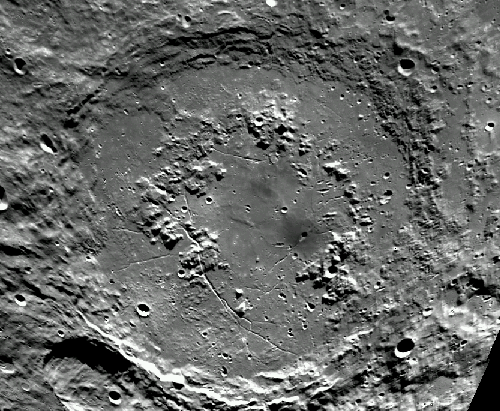
\includegraphics[width=\linewidth]{images/schrodinger.png}
\subcaption{\textit{Schr\"{o}dinger Crater, the Moon}. One of the largest impact craters on the Moon, with a diameter of 320km. At this size, an inner, peak ring is formed rather than a central peak. Image from NASA's Clementine MDIS instrument. Image credit: NASA. \url{http://www.nasa.gov/mission\_pages/Mini-RF/multimedia/}. Accessed on January 3rd, 2014. \label{fig:lunarcrater}}
\end{minipage}
\caption{An example of a simple crater (\protect\subref{fig:meteorcrater}), a  complex central peak crater (\protect\subref{fig:mercurycrater}), and a complex peak ring crater (\protect\subref{fig:lunarcrater}). \label{fig:simplecomplex}}
\end{figure*}

Depending on the size of the impactor, as well as the cohesion and gravity of the target, either a simple (Figure \ref{fig:meteorcrater}) or complex (Figure \ref{fig:mercurycrater} and \ref{fig:lunarcrater}) crater will form. A complex crater is always larger than a simple crater, but has a significantly smaller depth-to-diameter ratio. While a simple crater tends to be bowl shaped, a complex crater often has a flat crater floor with a central peak/peak ring. The rim of a complex crater consists of large terraced blocks of slumped material \citep{osinski2012impact}.

If a crater is large enough at the beginning of modification, it will become gravitationally unstable and collapse \citetext{e.g., \citet{melosh1999impact}}. For collapse to occur, numerical models require that the target rock must be weakened to a much greater extent than standard rock mechanics predicts \citep{mckinnon1978investigation}. Acoustic fluidisation \citep{melosh1979acoustic} is a model that attempts to explain this inferred weakening.

\subsection{The Full Model of Acoustic Fluidisation \label{sec:acfl}}

The full model of acoustic fluidisation, derived by \citet{melosh1979acoustic}, is a mechanical model which describes how temporally and spatially varying acoustic vibrations induce temporary weakening.

Acoustic vibrations are generated by the impact's shock wave and are scattered around the impact zone. These vibrations cause pressure fluctuations about the ambient overburden pressure. When the overall pressure drops below the ambient pressure the material's yield strength is reduced, resulting in temporary weakening. Thus, when target deformation is averaged over time and space, the rock material behaves as a viscous fluid. The equation that describes the yield strength of the acoustically fluidised rock material, $Y_{vib}$, is given as \citep{collins2003acoustic}:

\vspace{-0.1cm}
\begin{equation} \label{eq:yield_vib}
Y_{vib} = \eta_{\text{eff}} \dot{\epsilon} \approx  \frac{\rho \lambda c_{p}}{2 \psi} \left[ \frac{1+\erf\left(\chi\right)}{1-\erf\left(\chi\right)} \right] \dot{\epsilon}.\vspace{0.2cm}
\end{equation} 

The basic relationship involves the acoustically fluidised material's strain rate, $\dot{\epsilon}$, and effective viscosity, $\eta_{\text{eff}}$. The full definition of $\eta_{\text{eff}}$ is given on the far right hand side, where $\rho$ is the material's density, $\lambda$ is the wavelength of acoustic vibrations, and $\psi$ is the square of the compressional wave velocity divided by the shear wave velocity, $(c_{p}/c_{s})^{2}$. $\chi$ is defined as \citep{collins2002numerical}: 

\vspace{-0.2cm}
\begin{equation}\label{eq:chi}
\chi=\frac{s_{c}}{\sigma},
\end{equation}

where $s_{c}$ is the critical pressure amplitude for sliding to occur, and $\sigma$ is the variance of the vibrational pressure. $\sigma$ is equal to $c_{p} \rho \sqrt{2E}$, where E is the acoustic energy density (per unit volume). The velocity of the vibrations, $v_{vib}$, is related to the acoustic energy density via \citep{collins2002numerical},

\vspace{-0.2cm}
\begin{equation}\label{eq:velo}
v_{vib}=\sqrt{2E}.
\end{equation} 

The full equation that describes the temporally and spatially varying acoustic energy density per unit time is a non-linear, ordinary differential equation \citep{melosh1996dynamical}:

\begin{equation} \label{eq:dedt}
\frac{d E}{d t} = \frac{\xi}{4} \nabla^{2}E - \frac{c_{p}}{\lambda Q}E + e \tau_{ij} \dot{\epsilon}_{ij},\vspace{0.2cm}
\end{equation} 

where $\xi$ is the scattering diffusivity and $e$ is known as the regeneration parameter. $Q$ is the dissipation quality factor, formally defined as the  ratio of energy stored per cycle to the energy dissipated in that period \citep{collins2003acoustic,melosh1996dynamical}.

The first term on the right hand side of equation \ref{eq:dedt} describes scattering/diffusion of acoustic energy. The effect of the scatter term increases for smaller impacts because the length scale of scattering becomes large with respect to the crater size.
 
The second term describes the conversion of acoustic energy into heat per unit time, hence it is a positive value subtracted from the rate of change of acoustic energy density. It is known as the dissipation term, and is strongly dependent on the product $\lambda Q$. 

The final term in the differential equation acts to generate acoustic energy in regions with large stresses and strain rates. The regeneration parameter, $e$, holds a value between zero and unity, and influences the efficiency of acoustic energy regeneration \citep{melosh1996dynamical}. The term dictates how much distortional energy per unit time (given by $\tau_{ij} \dot{\epsilon}_{ij}$) is converted into acoustic energy.  Without the regeneration term, equation \ref{eq:dedt} would be linear and thus the solution behaviour would be relatively uninteresting. However, the regeneration term causes the equation to become very non-linear, which leads to interesting behaviour.

\subsection{The Block Oscillation Model}

The block model is a widely used alternative to the \citet{melosh1979acoustic} model of acoustic fluidisation. It is derived from a simplified situation of acoustic fluidisation, where a single block slides over a surface \citep{ivanov1997block}. It assumes that the acoustically fluidised region of the target is fractured into a series of large blocks, each separated by a matrix of smaller blocks. Acoustic vibrations, remnant from the impact's shock wave, cause the larger blocks to oscillate, decreasing the stress and coefficient of friction between the blocks and the matrix \citep{collins2002numerical,ivanov1997block}. Consequently, sliding is induced between the blocks.

The effective strength of the rock material for the block model, $Y_{\text{eff}}$, is given as:

\begin{equation}
Y_{\text{eff}}=\mu (p-p_{v}) + \eta_{\text{eff}} \dot{\epsilon}
\end{equation}

where $\mu$ is the coefficient of friction, $p$ is the overburden pressure and $p_{v}$ is the amplitude of the pressure vibrations from the sliding blocks \citep{ivanov1997block,melosh1999impact}. In contrast to the Melosh model, $\eta_{\text{eff}}$ is an input parameter rather than a function of acoustic energy. For the block model, it is assumed that $\eta_{\text{eff}}$ is proportional to impactor size. \citet{melosh1999impact} showed that the rheological effects of the block and Melosh models are similar. 

The block model, as implemented in the impact model used here, effectively solves equation \ref{eq:dedt} from the Melosh model for the case $e=0$ and $\xi=0$, so scattering and (re)generation of acoustic energy are never applied. Thus, the block model only solves the dissipation of acoustic energy. The initial distribution of acoustic vibrations, as implemented here, is based on the peak particle velocity of the target rather than through the regeneration term, thus initial acoustic vibrations follow the path of the shock wave. 

The block model fails to induce distinct, fault sized zones of localised weakening into hydrocode simulations \citep{kenkmann2012modification} because it neglects the scattering and, in particular, regeneration terms from equation \ref{eq:dedt}.

\subsection{The iSALE Hydrocode}

The impact model used to simulate crater formation in this research is known as iSALE, developed by Kai Wuennemann, Gareth Collins, and Dirk Elbeshausen. iSALE is a model for simulating flow at all speeds, including hypersonic flows and shock waves, otherwise known as a hydrocode \citep{collins2002numerical}. Essentially, a hydrocode calculates the sum of all forces acting at a node, and applies the corresponding acceleration to either the node or material within a cell, depending on an Eulerian or Lagrangian frame of reference, respectively. This process is carried out iteratively over all nodes in the model domain at incremental time steps. When the sum of all time steps reaches the final simulation time, the calculations stop \citep{collins2002numerical}.

iSALE is well suited for simulating asteroid impacts because it includes strength models that take into account the rheological properties of the medium. This is very important for impact cratering; the final, modified crater hugely depends on the rheology of the target, which may change depending on the size, velocity, and strength of the impactor, among other factors.


\section{Methodology}

\subsection{Energy Balance Solution}

In order to first implement the acoustic energy evolution equation (\ref{eq:dedt}) into iSALE, the acoustic energy density was converted to an energy per unit mass, using $\mathcal{E}_{v}=E/\rho$ \citep{collins2003acoustic}:

\begin{equation}\label{eqdedtmass}
\frac{d \mathcal{E}_{v}}{d t} = \frac{\xi}{4} \nabla^{2}\mathcal{E}_{v} - \frac{c_{p}}{\lambda Q}\mathcal{E}_{v} + e \frac{\tau \dot{\epsilon}}{2\rho}.\vspace{0.2cm}
\end{equation}

This is necessary, as iSALE stores specific energy rather than energy density.

To satisfy the conservation of energy, the energy available for regeneration of acoustic vibrations must be removed from the internal energy of the rock material. In iSALE, the rate of change of internal energy per unit mass, $I$, is given as \citep{collins2002numerical}:

\begin{equation}\label{eq:iSaleInternalEnergy}
\frac{d \left( \rho I\right)}{d t} =\frac{d \left(p + q\right)}{d t} + \tau \dot{\epsilon},\vspace{0.2cm}
\end{equation}

where the terms on the right hand side represents the work done against compression and deformation, respectively. To account for energy transfer, both the acoustic energy lost in heat dissipation and the amount of distortional energy available for acoustic regeneration must be included in equation \ref{eq:iSaleInternalEnergy}. This was achieved by adding the second term and one minus the third term from equation \ref{eqdedtmass} to equation \ref{eq:iSaleInternalEnergy} \citep{collins2002numerical}:

\begin{equation}\label{eq:iSaleInternalEnergyAcoustic}
\frac{d \left(\rho I\right)}{d t} =\frac{d \left(p + q\right)}{d t} + \tau \dot{\epsilon}\left(1-\frac{e}{2}\right)+\frac{c_{p}}{\lambda Q}\mathcal{E}_{v}.\vspace{0.2cm}
\end{equation}

Finally, the first term from equation \ref{eqdedtmass} must also be included to account for the scattering of acoustic energy \citep{collins2002numerical}. This is simply diffusion of acoustic energy, as governed by the Laplace equation:

\begin{equation} \label{eq:xydiff}
\frac{d \mathcal{E}_{v} }{d t} = \frac{\xi}{4} \left( \frac{d^{2} \mathcal{E}_{v}}{d x^{2}} +\frac{d^{2} \mathcal{E}_{v}}{d y^{2}} \right),\vspace{0.2cm}
\end{equation}

or, for a cylindrical coordinate system with angular symmetry about the z-axis;

\begin{equation} \label{eq:cyldiff}
\frac{d \mathcal{E}_{v} }{d t} = \frac{\xi}{4}  \left( \frac{1}{r} \frac{d}{dr} \left( r \frac{d \mathcal{E}_{v}}{dr} \right) + \frac{d^{2} \mathcal{E}_{v}}{dz^{2}}   \right) .\vspace{0.2cm}
\end{equation} 

Equations \ref{eqdedtmass}, \ref{eq:iSaleInternalEnergyAcoustic}, and \ref{eq:cyldiff}, as well as the acoustic fluidisation strength model (equation \ref{eq:yield_vib}) were successfully implemented into the iSALE hydrocode. This is further detailed in \ref{app:modifications}.

Verification of the scatter term subroutine implemented in iSALE was performed using an ideal model. The initial conditions described a sphere of high acoustic energy, surrounded by zero acoustic energy. In this situation, acoustic energy should diffuse/scatter into the sphere's surroundings. The error between the iSALE solution and a second order implicit finite difference solution, computed in Python, for several model resolutions is shown in (Figure \ref{fig:scatter_test}). This demonstrated that the scatter term was successfully implemented, with the iSALE solution showing a greater than first order rate of convergence.

\begin{figure}[!ht]
		\centering
		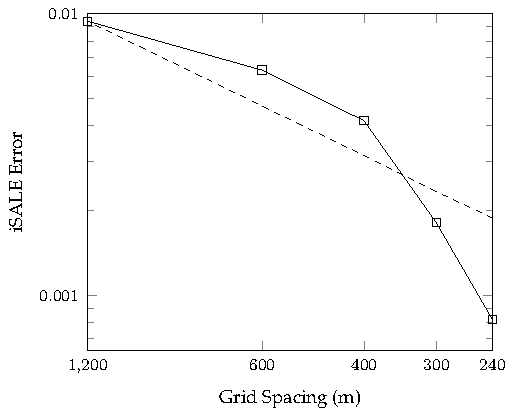
\includegraphics[width=\linewidth]{./images/scatter_test2.pdf}
		%\captionsetup{width=0.58\linewidth}
		\caption{Log-log plot of the error between the implicit finite difference and iSALE solutions to the scattering term in equation \ref{eqdedtmass}, with a test value of $\xi=10^{6}$ m$^2$ s$^{-1}$. The dashed line represents a first order convergence line with a slope of one. As the grid spacing is decreased (i.e., resolution is increased), the iSALE solution shows a greater than first order convergence.\label{fig:scatter_test}}
\end{figure}\vspace{-0.3cm}

\subsection{Models and their Parameters}\label{sec:parameters}

To test the implementation of the Melosh model and contrast its behaviour against the block model, three different sized scenarios of crater formation were created. Both acoustic fluidisation models were applied to each scenario on separate simulations. Table \ref{tb:ABC_table} displays all the acoustic fluidisation parameters used in each scenario, as well as the model setup parameters. Static model parameters are presented in Table \ref{tb:static}. The static strength of rock in each case was assumed to be the same.

\begin{table}[!t]
\small
\centering
\begin{tabular*}{\linewidth}{@{\extracolsep{\fill} }p{3cm} c c c}
\toprule
& \multicolumn{3}{c}{Scenario} \\ \cmidrule{2-4}
Parameter & A & B & C \\ \midrule
Impactor radius, $a$ (km) & 7.200 & 0.720 & 0.072 \\
Impactor resolution & 36 & 24 & 18 \\ 
Grid spacing (m) & 200 & 30 & 4 \\  
Scattering diffusivity, $\xi$ (m$^{2}$ s$^{-1}$) & 10$^3$ & 10$^3$ & 10$^3$ \\
Dissipation quality factor, $Q$ & 10-400 & 10-400 & 10-400 \\
Vibrational wavelength, $\lambda$ (m) & 1440-360 & 144-36 & 14.4-3.6 \\
Regeneration parameter, $e$ & 0.1 & 0.1 & 0.1 \\ \bottomrule
\end{tabular*}
\caption{Melosh model acoustic fluidisation parameters used in each crater formation scenario. Global parameters are given in Table \ref{tb:static}}\label{tb:ABC_table}
\end{table}

\begin{table*}[!bh]
\small
\centering

\begin{tabular*}{\linewidth}{@{\extracolsep{\fill} }p{2cm} l l}
\toprule
Parameter & Description & Value \\ \midrule
$g$ & acceleration of gravity & 9.81 m s$^{-2}$\\
$U$ & impactor velocity & 1.2 $\times$ 10$^{4}$ m s$^{-1}$\\
$T_{\text{melt}}$ & melting temperature & 1673 K \\  
$\mu_{\text{int}}$ & intact material internal coefficient of friction & 2.0 \\
$\mu_{\text{dam}}$ & damaged material internal coefficient of friction  & 0.6\\
$Y_{\text{int}}$& intact material yield strength  & 10$^7$ kg m$^{-1}$ s$^{-2}$\\
$Y_{\text{dam}}$& damaged material yield strength & 10$^4$ kg m$^{-1}$ s$^{-2}$\\
$mat_{\text{t}}$& target material type & granite\\
$mat_{\text{p}}$& impactor material type & granite\\
$\rho_{\text{t}}$ & target material density & 2630 kg m$^{-3}$\\ 
$\rho_{\text{p}}$ & impactor material density & 2630 kg m$^{-3}$ \\  \bottomrule
\end{tabular*}
\caption{Static model parameters used in all Melosh and block model scenarios.}\label{tb:static}
\end{table*}

The square of the compressional wave velocity divided by the shear wave velocity, $\psi$, was maintained at 10 throughout all simulations, following the reasoning provided by \citet{collins2003acoustic}. The single values for $e$ and $\xi$ used here were selected from the range of possible values demonstrated by \citet{collins2003acoustic} in their work simulating the mobility of large rock avalanches. 

The two main parameters that were varied, as shown in Table \ref{tb:ABC_table}, were the vibrational wavelength, $\lambda$, and the quality dissipation factor, $Q$. Both of these are somewhat unconstrained, as are all the parameters in the Melosh model. However, $Q$ has the best constraint as it is similar to another parameter, the seismic $Q$ \citep{melosh1996dynamical}. A typical value of the seismic $Q$ in the upper crust is 500 \citep{anderson1989theory}, which accounts for both elastic energy converted to heat and scattering. In contrast, the Melosh model $Q$ only includes conversion to heat, thus 500 is likely an underestimate. \citet{melosh1999impact}, however, demonstrated that $Q$ must be of the order 10-100 for block model results to realistically fit observed crater profiles. As such, $Q$ was varied between 10-400 in this study. 

The only constraint set on the vibrational wavelength, $\lambda$, is that it must be less than the final crater diameter, but much greater than the material grain size \citep{melosh1979acoustic,collins2002numerical}. In accordance with this, $\lambda$ was assumed to scale proportionally with impactor size \citep{collins2003acoustic}. The block model makes a similar assumption, in that block size is also proportional to impactor size \citep{ivanov1997block}. This assumption is key: if $\lambda$ decreases with decreasing impactor size, the dissipation term in equation \ref{eqdedtmass} will become large, thus acoustic energy will dissipate more rapidly for smaller impacts. Consequently, $\lambda$ was maintained as a fraction of the impactor radius, ranging from $0.2a$ to $0.05a$.

The block model parameters used were similar to typical parameters used in recent work \citetext{e.g., \citet{wunnemann2003numerical}}. 


\section{Results \label{sec:results}}

\begin{figure*}[!b]
\centering
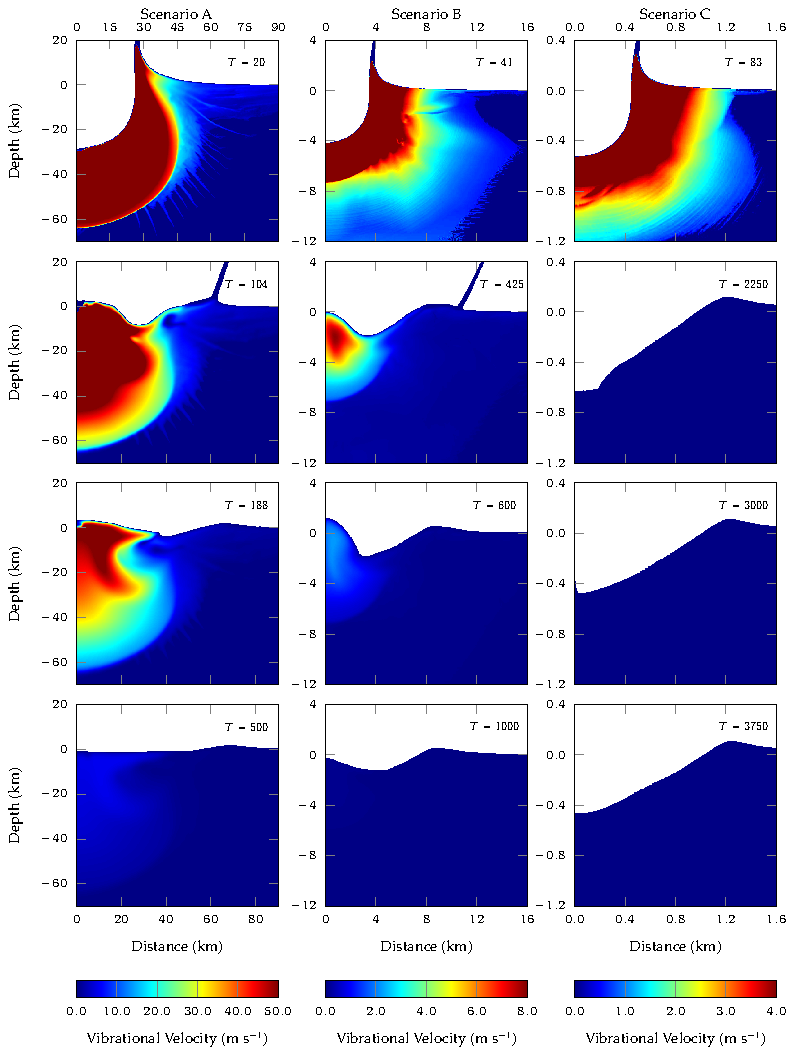
\includegraphics[width=0.7\linewidth]{./images/block_velo.pdf}
\caption{The evolution of acoustic vibrations for the block model in scenarios A, B and C. The zone of intense vibrations decreases in size as vibrations decay after the initial distribution of acoustic energy. This occurs the fastest in scenario C. Decay is strongest laterally in scenarios A and B. Note the different colour scales used here. \label{fig:block_velo}}
\end{figure*}

Crater formation time is greatest for large impacts. Consequently, it is difficult to compare crater formation stages for impacts of different sizes. The approach used here is to non-dimensionalise time using the shock wave propagation time, which is approximately proportional to impactor size divided by velocity. Thus the non-dimensional time $T$ is related to time via:

\begin{equation}
T=\frac{Ut}{a}
\end{equation}

where $U$ is the impactor velocity, $t$ is the simulation time in seconds, and $a$ is the impactor radius \citep{o1993planetary}.

Several non-dimensional time slices showing the evolution of acoustic vibrations for the block and Melosh models are shown in figures \ref{fig:block_velo} and \ref{fig:melosh_velo}, respectively. Scenarios A, B and C are shown from left to right in both figures.

\subsection{Block Model Evolution of Acoustic Vibrations}\label{sec:blockvelo}

\begin{figure*}[!b]
\centering
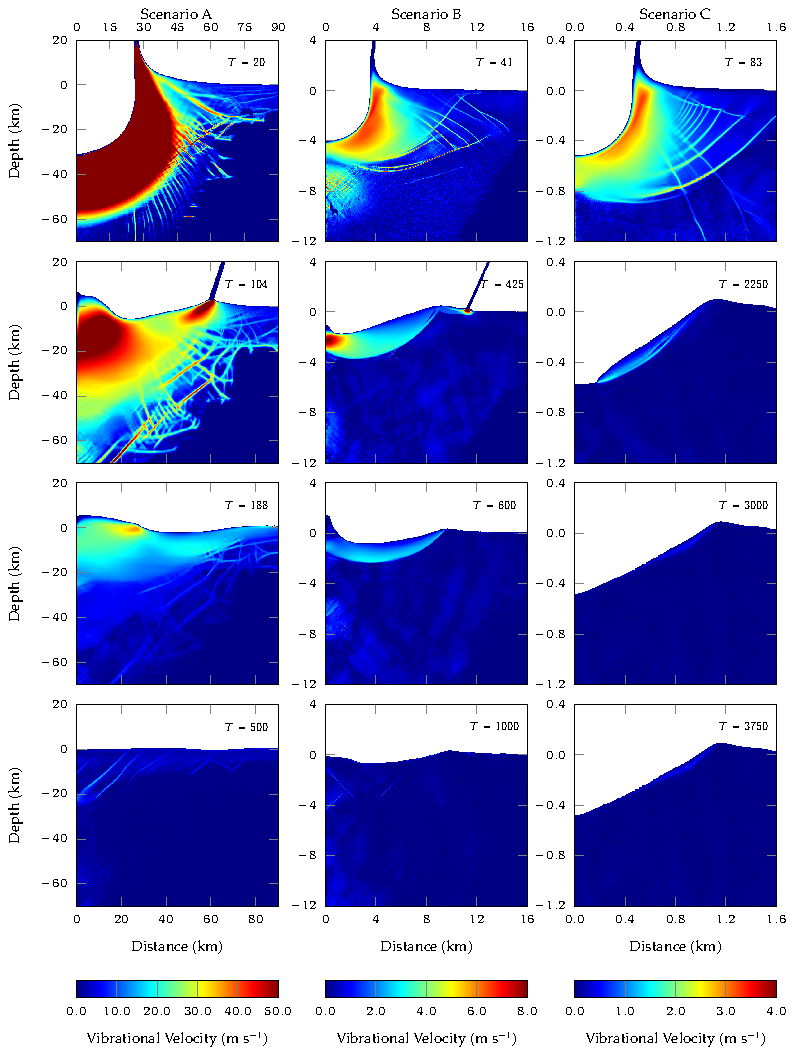
\includegraphics[width=0.7\linewidth]{./images/melosh_velo.pdf}
\caption{The evolution of acoustic vibrations for the Melosh model in scenarios A, B and C. Localised regions of vibrational velocity are evident throughout all scenarios. As in the block model, the rate of acoustic dissipation increases from scenarios A to C, where vibrations dissipate the fastest. Decay is strongest vertically in scenarios A and B. There is also significant regeneration of acoustic vibrations in localised regions of the domain. Note the different colour scales used here. $\lambda=0.2a$ and $Q=10$. \label{fig:melosh_velo}}
\end{figure*}

\begin{figure*}[!t]
\centering
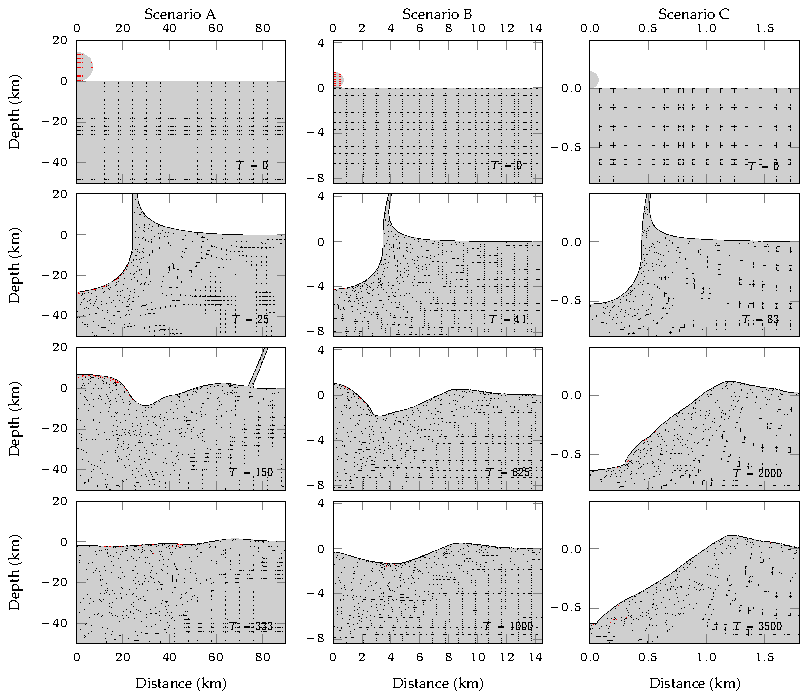
\includegraphics[width=0.99\linewidth]{./images/block_deformation.pdf}
\caption{Evolution of subcrater deformation in the block model for scenarios A, B and C. The style of deformation is much the same for the second time slice across all scenarios. Scenarios A and B both show large central uplifts in the third time slice, while the bottom of the transient crater in scenario C does not rebound at all. All scenarios show inward rim collapse in the third time slice. \label{fig:block_deformation}}
\end{figure*}


\begin{figure*}[!t]
\centering
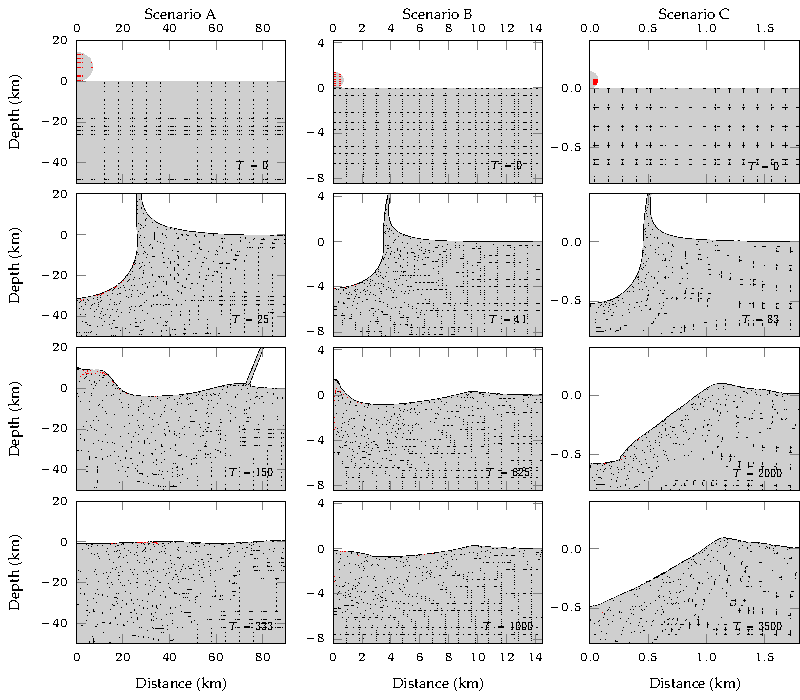
\includegraphics[width=0.99\linewidth]{./images/melosh_deformation.pdf}
\caption{Evolution of subcrater deformation in the Melosh model for scenarios A, B and C. As in the block model, the style of deformation is very similar for all three scenarios at the second time slice. Scenario A  has a much wider central uplift than B in the third time slice. All scenarios show inward rim collapse in the third time slice. $\lambda=0.2a$ and $Q=10$. \label{fig:melosh_deformation}}
\end{figure*}



%\newgeometry{top=1.5cm,bottom=2cm,left=4cm,right=2.5cm}

\begin{figure*}[!t]
\centering
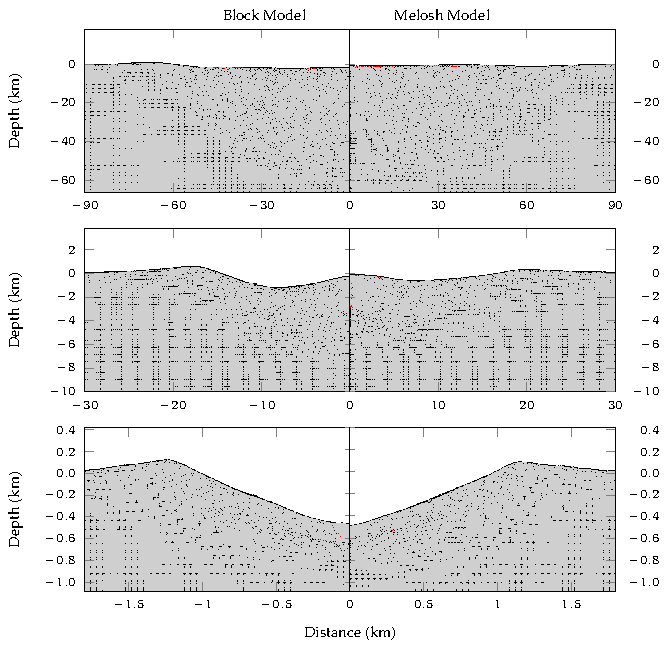
\includegraphics[width=0.8\linewidth]{./images/comparison.pdf}
\caption{A comparison of all final crater morphologies using the block (left) and Melosh (right) models of acoustic fluidization for scenarios A (top), B (middle) and C (bottom). Both models produce similar crater morphologies for their respecitve scenarios; a peak ring complex crater in scenario A, a central peak crater in scenario B, and a simple crater in scenario C. $\lambda=0.2a$ and $Q=10$ for the Melosh model. \label{fig:comparison}}
\end{figure*}

\begin{figure*}[!t]
\centering
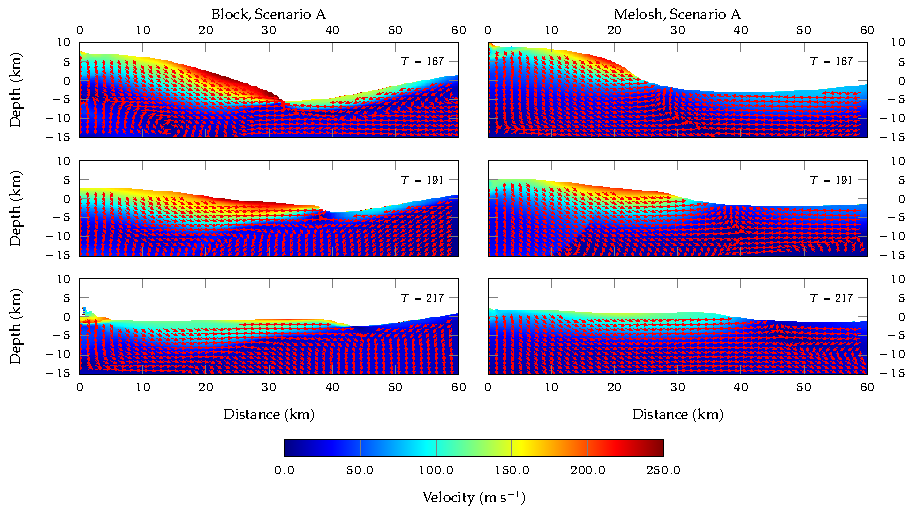
\includegraphics[width=\linewidth]{./images/peak_ring.pdf}
\caption{A comparison of velocity vectors during peak ring formation between the block and Melosh models for scenario A. It is evident that rock material is forced under the outwardly collapsing inner material for the block model. In the Melosh model, however, inwardly collapsing material is forced up against the outardly collapsing material, forming a central peak at the confluence between the two. $\lambda=0.2a$ (7200m) and $Q=10$.\label{fig:peak_ring}}
\end{figure*}

The broad, spatial characteristics of the initial vibrational velocity field for all scenarios in the block model (Figure \ref{fig:block_velo}) show deep zones of intense acoustic vibrations ($v_{vib} > 50$ m s$^{-1}$). At no point in any scenario are vibrations focused or localised into any region of the domain. After the shock wave has passed in the second and third time slices, the zone of intense vibrations  begins to decay, shrinking in size. In scenario A, the strongest decay occurs laterally, causing intense vibrations to persist at depth in the third time slice. Strong lateral decay in scenario B also reduces intense vibrations into a small area centred directly inside the central uplift, as in scenario A. Decay occurs the fastest in the smallest scenario, C. 

Intense acoustic vibrations are not evident at the edge of the crater during the second and third time slices in any scenario. This is particularly important in scenarios A and B, which require a collapsed rim to form a complex crater.

Crater formation ends in the fourth time slice, when all vibrations have ceased.

\subsection{Melosh Model Evolution of Acoustic Vibrations}\label{sec:meloshvelo}

In some respects, the initial, broad, spatial variation in vibrational velocity in the Melosh model in Figure \ref{fig:melosh_velo} is much like that of the block model, particularly for scenario A. Again, intense vibrations extend deep into the target, although the magnitude of the vibrational velocity in scenarios B and C is much less than that in the block model. The most important difference, however, is the presence of localised vibrations in all scenarios of the Melosh model. 

In the second time slice, the size of the zone of intense vibrations decays faster than in the block model, and as a result is smaller in size. In contrast to the block model, decay occurs primarily in the vertical direction. A significant number of localised vibrations are also regenerated near the surface, particularly around the crater rim and central uplift in scenarios A and B.

There are significant acoustic vibrations laterally in the third time slice for the largest two scenarios, with vibrations spanning from the crater center to the crater rim. As in the block model, vibrations decay the fastest for scenario C.

\subsection{Subcrater Deformation \label{subsec:comparison}}

Figures \ref{fig:block_deformation} and \ref{fig:melosh_deformation} show the evolution of subcrater deformation in a series of time slices for the block and Melosh models, respectively. The dashed lines represent tracer particles, tracking the movement of rock material from its pre-impact position. The first time slice shows the initial condition of each model - the point at which contact and compression begins. The second time slice, taken during excavation, shows little difference in subcrater deformation in all scenarios, for both the block and Melosh models alike.

However, a range of differences in subcrater deformation arise in the third time slice, during modification. In scenario A, both models form a large central uplift. Radially, the block model's central uplift is around 10km larger than the Melosh uplift.

In scenario B, at time slice $T=625$, both models again form a large central uplift. Material existing just outside of the uplift core is primarily that which is uplifted into the developing central peak for the Melosh model. This contrasts with the block model, where central uplift material mostly originates from directly below the point of impact. As in scenario A, the central uplift is largest in the block model by $\sim$ 3km.

There is very little difference between the Melosh and block models in the final two time slices of scenario C. Both show displaced material collapsing back into the centre of the crater, forming a steep sided simple crater. 

A comparison of final crater morphology and subcrater deformation between the two models is shown in Figure \ref{fig:comparison}. Again, there is little difference between the two models in scenario C. The Melosh model produces a shallower crater in scenario B, and it is also evident that the vertical extent of subcrater deformation is smaller  than in the block model. This is especially true in scenario A.

The differing particle velocity fields for both models during peak ring formation in scenario A suggest two different modes of peak ring formation (Figure \ref{fig:peak_ring}). In the block model, central rock material collapses outwards on top of the inwardly collapsing rim. However, in the Melosh model, inwardly collapsing material is forced up against the outwardly collapsing material.


\section{Discussion \label{sec:discussion}}

\subsection{Complex Crater Collapse} 

The impact in scenarios A and B forms a complex crater for both acoustic fluidisation models (Figure \ref{fig:comparison}). In order for this to happen, wholesale crater collapse must occur. Both models induce enough weakening to achieve this, but the style of weakening differs between the two.

As described in sections \ref{sec:blockvelo} and \ref{sec:meloshvelo}, the spatial characteristics of acoustic energy are different in the two models. In the block model, for scenarios A and B, dissipation of acoustic energy mainly occurs laterally (Figure \ref{fig:block_velo}). The longevity of intense vibrations is thus greatest vertically, inferring that complex crater collapse is induced by a deep weakening, centered mainly under the central uplift. This is reinforced through the subcrater deformation in scenarios A and B; the central uplift in A is very large, and extends deep into the target (Figure \ref{fig:block_deformation}). The lateral extent of vibrations is still enough, however, to produce a wide central uplift. 

The lack of acoustic vibrations at the crater rim during modification in the block model (Figure \ref{fig:block_velo}) suggests that crater rim collapse is not a direct consequence of acoustic vibrations. This may be one of the reasons why the block model fails to produce discrete, terraced fault blocks at the crater rim in numerical simulations of crater collapse \citep{kenkmann2012modification}.

In the Melosh model, rapid vertical decay of vibrations removes intense vibrations from depth  in both scenarios A and B (Figure \ref{fig:melosh_velo}). Yet, crater collapse still occurs, suggesting that collapse is facilitated by shallow acoustic vibrations. Again, this is reinforced by the large, shallow, deformation shown in Figure \ref{fig:melosh_deformation}. Importantly, a large amount of acoustic energy is regenerated in scenarios A and B, particularly under the central uplift and crater rim at shallow depths. Shallow regeneration of acoustic energy in these areas also results in crater collapse for this set of acoustic fluidisation parameters. This is in contrast to the block model, where no regeneration of acoustic energy and deep weakening result in collapse.

\subsection{Crater Morphology}

\begin{table}[!t]
\small
\centering
\begin{tabular*}{\linewidth}{@{\extracolsep{\fill} }p{1.5cm} c c c c}
\toprule
& \multicolumn{4}{c}{Dimension} \\ \cmidrule{2-5}
Crater & $D$ (km) & $d$ (km) & $d/D$ & $d_{s}$ (km) \\ \midrule
Block, A & 113 & 0.948 & 0.0084 & 1.145$^b$\\
Melosh, A & 154 & 0.596 & 0.0039 & 1.308$^b$\\ \midrule
Block, B & 14.8 & 0.345 & 0.0233 & 0.478$^b$\\
Melosh, B & 17.2 & 0.146 & 0.0085 & 0.510$^b$\\ \midrule
Block, C & 2.06 & 0.464 & 0.2256 & 0.407$^a$\\
Melosh, C & 1.97 & 0.474 & 0.2408 & 0.389$^a$\\ 
\bottomrule
\end{tabular*}
\caption{Table of crater dimensions for all scenarios. $D$ = diameter, $d$ = depth, and $d_{s}$ = scaling law depth. Scaling law a; \citet{pike1977apparent}, b; \citet{grieve1992terrestrial}}.\label{tb:crater_dimensions}
\end{table}

Both models produce similar crater morphologies for each scenario, as shown in Figure \ref{fig:comparison}. While the craters formed are of the same type, their depth and diameter differ. Table \ref{tb:crater_dimensions} shows crater depth, $d$, scaling law depth, $d_{s}$, diameter, $D$, and depth-to-diameter ratio for all block and Melosh model scenarios. 

Similar crater dimensions are formed by both models for the simple crater in scenario C. As discussed earlier, the deformation and vibrational velocity field are also very alike in this scenario. At this scale and for this set of parameters, the block and Melosh models produce very similar results.

\begin{figure*}[bp]

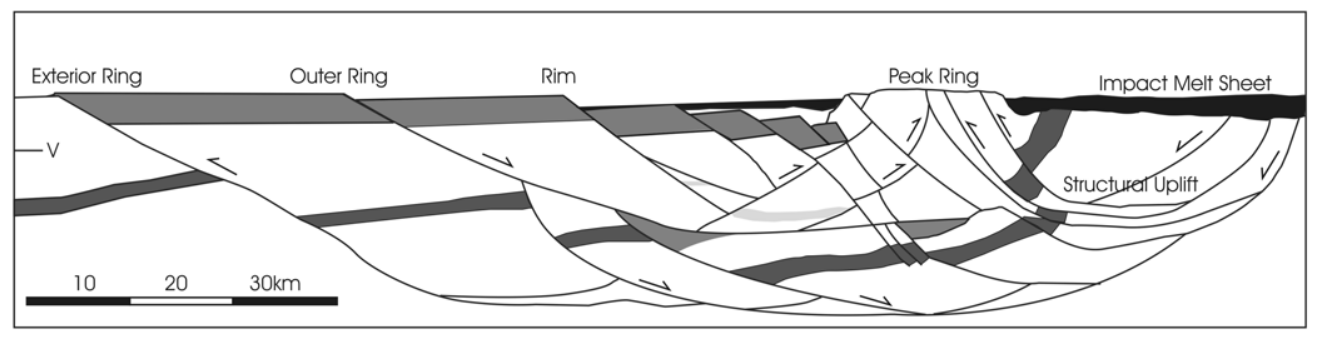
\includegraphics[width=\linewidth]{images/grieve_model.png}
\caption{Structural model of the peak rings at Vredfort, Chicxulub and Sudbury craters from \citet{grieve2008observations}. Here the the peak ring is formed at the confluence of inwardly and outwardly collapsing material. This model is, however, inconsistent with seismic observations at Chicxulub \citep{morgan2011full}, where outer ring material is forced directly under the forming peak ring.}\label{fig:grieve_model}
\end{figure*}

The depth and diameter scaling law for simple craters used in Table \ref{tb:crater_dimensions} \citep{pike1977apparent}:

\vspace{-0.2cm}
\begin{equation}\label{eq:simple_scaling}
d=0.196 D^{1.01},
\end{equation}

yields similar crater depths for both models in scenario C. The model depths are very similar to those predicted by the scaling law, although the block model is a closer approximation.

In scenario A similar crater dimensions are formed in both models, but as is obvious from Figure \ref{fig:comparison}, the crater diameter is considerably larger in the Melosh model and the depth is smaller. Overall, this results in a depth-to-diameter ratio that is smaller than the block model, but still the same order of magnitude.

The greatest difference in crater morphology, both quantitatively and qualitatively, is in scenario B. This is evident from both Table \ref{tb:crater_dimensions} and Figure \ref{fig:comparison}. The depth-to-diameter ratio differs by an order of magnitude between the two models. The Melosh model takes the smaller value, similar to the depth-to-diameter ratios recorded in scenario A.

A scaling law developed by \citet{grieve1992terrestrial} for complex craters in crystalline targets:

\vspace{-0.2cm}
\begin{equation}\label{eq:complex_scaling}
d=0.15 D^{0.43},
\end{equation}

is compared to the block and Melosh models for scenario B. The recorded block model depth is approximately 100m shallower than that predicted by the scaling law, whereas the Melosh model is around 300m shallower. Again, the block model produces the better approximation.

The scaling laws applied here are not perfect. They are based on terrestrial crater data, which is, due to erosion, poor at best. For simple craters, the two models agree very well with the scaling laws, each producing craters around 400m deep. The block model depths for complex craters are also reasonably close, differing by 100-200m from the scaling law. However, the Melosh model produces complex craters that are up to 700m shallower than that predicted by the scaling law. Thus, for this set of parameters, the Melosh model consistently underestimates complex crater depth while the block model produces a close approximation. This is perhaps unsurprising given how little the Melosh model has been tested when compared to the block model.

\subsection{Peak Ring Formation}

Both the block and Melosh models for scenario A form a peak ring. However, there is some debate as to quite how peak rings form in complex craters, as observational evidence has lead to conflicting mechanisms. 

The block model results presented here are similar to hydrocode simulations performed by \citet{collins2002hydrocode} and \citet{ivanov2005numerical}. Simulations of Chicxulub crater formation indicate that the inwardly collapsing crater rim is forced underneath the outwardly collapsing central uplift, forming the inner peak ring \citep{collins2002hydrocode}. These results agree well with seismic observations of the peak ring and its internal structure at Chicxulub \citep{morgan2011full}. Inward dipping reflectors are interpreted from the seismic data, indicating that inwardly collapsing crater material is indeed forced underneath the forming peak ring. The block model velocity field shown in Figure \ref{fig:peak_ring} supports this observation, reinforcing an already well known mechanism for peak ring formation.

\citet{grieve2008observations} observed structural evidence for an alternative mechanism of peak ring formation at Vredfort crater, South Africa (Figure \ref{fig:grieve_model}). The 120-200km diameter impact crater \citep{turtle2005impact} is one of the biggest on Earth, and has the morphology of a complex, peak ring impact crater. The structural model of a terrestrial ring basin produced by \citet{grieve2008observations}, shown in Figure \ref{fig:grieve_model}, is one which suggests that the peak ring is a result of uplift at the confluence of inwardly and outwardly collapsing crater material. The velocity field during peak ring formation for the Melosh model in scenario A (Figure \ref{fig:peak_ring}) suggests that this mechanism may well be a viable one. This also enhances the credibility of the Melosh model presented here.

The relative timing of when material outside and inside the peak ring begin to collapse may be key in deciding which of the two mechanisms comes into play during peak ring formation \citep{grieve2008observations}. Certainly, the observations from Chicxulub and Vredfort discussed above suggest that either mechanism may be relevant for peak ring formation. As the block model favours observations from Chicxulub, while the Melosh model favours observations from Vredfort, it is difficult to say which model produces the 'better' approximation. Clearly, a study of Chicxulub and Vredfort crater formation using both the block and Melosh models would be useful. 


\subsection{Melosh Model Parameter Space and Sensitivity}

To sufficiently weaken the target rock for any length of time, it was found that  $\lambda$ could be as high as $0.2a$. As $\lambda$ decreases with impactor radius, the rate of dissipation increases, as described in section \ref{sec:parameters}. This results in faster acoustic energy dissipation for smaller impacts. However, making $\lambda$ too small ($0.05a$) resulted in complex craters being formed in scenarios A, B and C, which is unrealistic for terrestrial impacts. This is because the effective viscosity, $\eta_{\text{eff}}$, is proportional to $\lambda$ (equation \ref{eq:yield_vib}).

There exists a trade-off between the longevity of vibrations, governed by $\lambda Q$, and the magnitude of weakening, governed primarily by $\lambda$. A comprehensive study of $\lambda$ and $\lambda Q$ parameter space would be useful in determining how variations in these two parameters influence crater morphology and subcrater deformation. Realistically, the value of $Q=10$ used here is at least an order of magnitude too small \citep{melosh1996dynamical,anderson1989theory}. However, the product $\lambda Q$, where $Q=10$ and $\lambda = 0.2a$, is small enough that complex craters are formed in scenarios A and B, and not in C (Figure \ref{fig:comparison}). If $\lambda Q$ is an order of magnitude bigger, the dissipation term becomes so small that, again, complex craters are created in all three scenarios as vibrations do not dissipate fast enough.

To increase $Q$ by an order of magnitude, $\lambda$ must decrease by an order of magnitude (i.e., $0.01$-$0.02a$). This is not possible with the current model, as $\lambda$ would become smaller than the cell size and thus spatial variations in acoustic energy would not be fully resolved. As such, this is a problem regarding resolution. By increasing the resolution these changes to $\lambda$ and $Q$ could be tested. Given the non-linearity of the Melosh model, however, it is hard to say if these parameter changes will result in the predicted crater morphologies for all three scenarios. Clearly, this is an area for further study.

\section{Conclusions}

This work demonstrates the successful implementation of the full Melosh model of acoustic fluidisation into the iSALE hydrocode. The Melosh model results presented here agree with the predicted evolution of acoustic energy in both space and time \citep{melosh1979acoustic}. A series of results that explore a small region of the Melosh model parameter space are also presented and compared to an alternative, widely used approximation of acoustic fluidisation - the block oscillation model. Certain values of these parameters are shown to produce predicted crater morphologies for a range of terrestrial impacts, from simple craters to peak ring complex craters. However, Melosh model crater depths deviate more strongly from terrestrial scaling laws for complex craters than do those of the block model.

Crater collapse in the Melosh model is facilitated by the shallow regeneration of localised acoustic energy, while collapse in the block model is the result of long lived vibrations extending deep into the target. Localised, shallow acoustic vibrations in the Melosh model result in different styles of subcrater deformation between the two models. In particular, the two acoustic fluidisation models predict different modes of peak ring formation that correspond to alternative hypothesis based on observational evidence. To further explore the differences between the two models, an extensive exploration of Melosh model parameter space at high resolution is required, as well as a detailed comparison of subcrater deformation between the two models and observational evidence. 

\section*{References}
\bibliography{msci_biblio}

\appendix

\section{Modifications to iSALE} \label{app:modifications}

To apply the Melosh model in the iSALE hydrocode, two main algorithms were applied to the iSALE time loop: (1) (re)generation and movement of acoustic energy, and (2) the effect of acoustic vibrations on the strength of the rock medium.

\subsubsection{Dissipation and Regeneration \label{sec:dissandregen}}

iSALE updates each cell's energy value at every new timestep using the stored values from the previous timestep, hence, at timestep number $n$:

\begin{equation}\label{eq:iSaleStep}
\mathcal{E}_{v_{n}} = \mathcal{E}_{v_{n-1}} + d\mathcal{E}_{scatter} + d\mathcal{E}_{dissipation} + d\mathcal{E}_{regeneration},\vspace{0.2cm}
\end{equation}

where $d\mathcal{E}_{scatter}$, $d\mathcal{E}_{dissipation}$, and $d\mathcal{E}_{regeneration}$ represent the three terms on the right hand side of equation \ref{eqdedtmass} respectively \citep{collins2003acoustic}.

The dissipation and regeneration terms were relatively simple to compute in the iSALE code, evaluated as follows:
\vspace{0.0cm}
\begin{eqnarray}
d\mathcal{E}_{dissipation} &=& \frac{c_{p}}{\lambda Q}\mathcal{E}_{v_{n-1}}\, dt \\
d\mathcal{E}_{regeneration} &=& De \frac{\tau \dot{\epsilon}}{2\rho}\, dt\, . \label{eq:regen_term}
\end{eqnarray}


$D$ represents the damage parameter; a value between zero and unity which describes how 'damaged' the rock material is \citep{collins2004modeling}. In this case, it acts to switch off generation of acoustic energy. For a region of undamaged material: when $D=1$, damage is at a maximum, and therefore so is $d\mathcal{E}_{regeneration}$.

For each cell, the internal energy was also updated as energy became available for regeneration. This was done by adapting equation \ref{eq:iSaleInternalEnergyAcoustic} to give the internal energy of each cell at timestep number $n$:

\begin{equation}\label{eq:internalEnergydt}
I_{n} = I_{n-1} + \frac{1}{\rho}\left[\frac{d \left(p + q\right)}{d t} + \tau \dot{\epsilon}\left(1-\frac{e}{2}\right)+\mathcal{E}_{dissipation}\right] dt.\vspace{0.2cm}
\end{equation}
 
Small stresses and strain rates may result in the generation of acoustic energy, as equation \ref{eq:regen_term} predicts. However, regions with extremely low strain rates far away from the point of impact would normally be mostly unaffected by the impact. To restrict acoustic fluidisation in these areas, a strain rate limit of $3\times10^{-3}$ s$^{-1}$ was set, i.e., for a cell with a strain rate lower than this value, $d\mathcal{E}_{regeneration}=0$.

\subsubsection{Scattering \label{sec:scatter}}

As iSALE can either use cartesian or cylindrical coordinates when run in 2D, it was important to provide a convenient method for switching the Laplace equation in the scattering term between these two coordinate systems. This was achieved by using a binary variable $cyl$, used in iSALE. $cyl$ takes the value of either 0 or 1, representing a cartesian or cylindrical coordinate system respectively.

The full expansion of the scatter term in cylindrical coordinates (equation \ref{eq:cyldiff}) was derived using the product rule, giving:

\begin{equation}\label{eq:scatter_expand}
\frac{d \mathcal{E}_{v} }{d t} = \frac{\xi}{4} \left(\frac{1}{r} \frac{d \mathcal{E}_{v}}{dr} + \frac{d^{2} \mathcal{E}_{v}}{dr^{2}} + \frac{d^{2} \mathcal{E}_{v}}{dz^{2}} \right),\vspace{0.2cm}
\end{equation}

where $r$ and $z$ are the cylinder radius and height, respectively. Applying the $cyl$ variable to this results in a convenient switch between the cartesian and cylindrical form of the Laplace equation:

\begin{equation}
\frac{d \mathcal{E}_{v} }{d t} = \frac{\xi}{4} \left(cyl\,\frac{1}{r} \frac{d \mathcal{E}_{v}}{dr} + \frac{d^{2} \mathcal{E}_{v}}{dr^{2}} + \frac{d^{2} \mathcal{E}_{v}}{dz^{2}} \right),\vspace{0.2cm}
\end{equation}

where $r$ and $z$ become $x$ and $y$ for a cartesian coordinate system. When $cyl=0$, the $1/r$ term is dropped. If $cyl=1$, then equation \ref{eq:scatter_expand} remains as it is. Thus, the scatter term becomes:

\begin{equation}
\mathcal{E}_{scatter} = \frac{\xi}{4} \left(cyl\,\frac{1}{r} \frac{d \mathcal{E}_{v}}{dr} + \frac{d^{2} \mathcal{E}_{v}}{dr^{2}} + \frac{d^{2} \mathcal{E}_{v}}{dz^{2}} \right)dt,\vspace{0.2cm}
\end{equation}

where it is added to the new specific acoustic energy, as in equation \ref{eq:iSaleStep}.

\subsubsection{Strength Model \label{sec:strength}}

\begin{sloppypar}
The effect of acoustic fluidisation on the rock strength, discussed in section \ref{sec:acfl}, was implemented in the \citet{collins2004modeling} strength model. iSALE updates the yield strength, $Y$, of the cells according to the user selected strength model at every time step. Yield strength is defined as:
\end{sloppypar}

\begin{equation} \label{eq:yield}
Y=\mu p, \vspace{0.2cm}
\end{equation}

where $\mu$ is the coefficient of friction, and $p$ is the overburden pressure. The critical pressure amplitude for sliding to occur, $s_{c}$, is defined as:

\begin{equation}
s_c=p -\frac{\tau}{\mu}
\end{equation}

Then multiplying this through by $\mu$ yields:

\begin{equation}
\mu s_c =\mu p - \tau. \vspace{0.2cm}
\end{equation}

By substituting in equation \ref{eq:yield}, this is then equivalent to:

\begin{equation}
\bar{Y}  =Y - \tau, \vspace{0.2cm}
\end{equation}

where $\bar{Y}$ is the critical yield stress for sliding to occur at pressure amplitude $s_c$. This can be arranged further to give the vibrational strength (the yield strength of the material as a result of acoustic vibrations):

\begin{equation}
Y_{vib} = Y - \bar{Y} = \tau. \vspace{0.2cm}
\end{equation} 

Finally, using the definition of $\eta_{\text{eff}}$ \citep{collins2003acoustic} and the basic relationship between stress and strain rate, $\tau = \eta \dot{\epsilon}$, gives:

\begin{equation} \label{eq:y_vib}
Y_{vib} = \eta_{\text{eff}} \dot{\epsilon} \approx  \frac{\rho \lambda c_{p}}{2 \psi} \left[ \frac{1+\erf\left(\chi\right)}{1-\erf\left(\chi\right)} \right] \dot{\epsilon}.\vspace{0.2cm}
\end{equation} 

iSALE then either used the yield strength of the material, $Y_{mat}$, or the yield strength from vibrations, $Y_{vib}$, depending on which value was smallest. This is because, although acoustic vibrations may temporarily cause strengthening, $Y_{vib}$ should never be greater than $Y_{mat}$.

A feature of equation \ref{eq:y_vib} is that as the strain rate decreases, so does the vibrational strength of the rock material. This results in significant weakening of material  in regions where the strain rate is very low. Thus, features far away from the impact may have a lowered strength due to a very slow rate of surface deformation. To avoid this, the same strain rate cut off variable that was used in \ref{sec:dissandregen} was applied here. If a cell's strain rate value was below this cut off value, no acoustic weakening of the cell would occur. This helped to avoid complete fluidisation of the rock material. 

\end{document}
